\section{Random Processes}
%% subsection
\subsection{Statistical Descriptions of Noise and Random Processes}
Noise signals cannot be described analytically. However, noise realizations in a specific condition share some \textit{statistical} properties. \\

\textbf{Random process} is the collection of \textbf{random variables}, denoted by $\mathbf{x}_n$. The theory of probability can characterise random variables.

\paragraph{Probability Distribution Function} A random variable is characterized by its probability distribution function, $F_{\mathbf{x}_n}(\alpha, n)$,
\[
    F_{\mathbf{x}_n}(\alpha, n) = P\{\mathbf{x}_n\leq \alpha\}.
\]
Note that the probability density function increases monotonically with $\alpha$.

\paragraph{Probability Density Function} If $\mathbf{x}_{n}$ takes a continuous range of values, it can also be characterized by the probability density function, $f_{\mathbf{x}_n}(\alpha, n)$,
\[
    f_{\mathbf{x}_n}(\alpha, n) = \frac{\partial F_{\mathbf{x}_n}(\alpha, n)}{\partial \alpha}.
\]
%% subsubsection
\subsubsection{Mean and Variance of a Distribution}
\begin{enumerate}
    \item The probability density between the range $a$ and $b$ is found
        \begin{align*}
            P \{a \leq \mathbf{x}_n \leq b \} 
            & = \int_{a}^{b} f_{\mathbf{x}_n} (\alpha, n) \ \mathrm{d} \alpha \\
            & = F_{\mathbf{x}_n}(b, n) - F_{\mathbf{x}_n}(a, n).
        \end{align*}
        For $a = -\infty$ and $b = +\infty$,
        \[
            P \{-\infty \leq \mathbf{x}_n \leq +\infty \} = \int_{-\infty}^{+\infty} f_{\mathbf{x}_n} (x, n) \ \mathrm{d} x = 1
        \]

        \begin{ex}{Uniform distribution}
        \label{ex:uniform_dist}
            Consider the probability density function of a uniform distribution described as
            \[
                f_{\mathbf{x}_n} (\alpha, n) = 
                \begin{cases}
                    \frac{1}{b-a}, & a \leq \alpha \leq b \\
                    0, & \text{otherwise}
                \end{cases}, 
            \]
            the corresponding probability distribution is
            \[
                F_{\mathbf{x}_n} (\alpha, n) = 
                \begin{cases}
                    0, & a < 0 \\
                    \frac{1}{b-a}(\alpha-a), & a \leq \alpha \leq b \\
                    1, & \alpha > b
                \end{cases}.
            \]
            As shown in \autoref{fig:uniform_dist}.
            \begin{figure}[H]
                \centering
                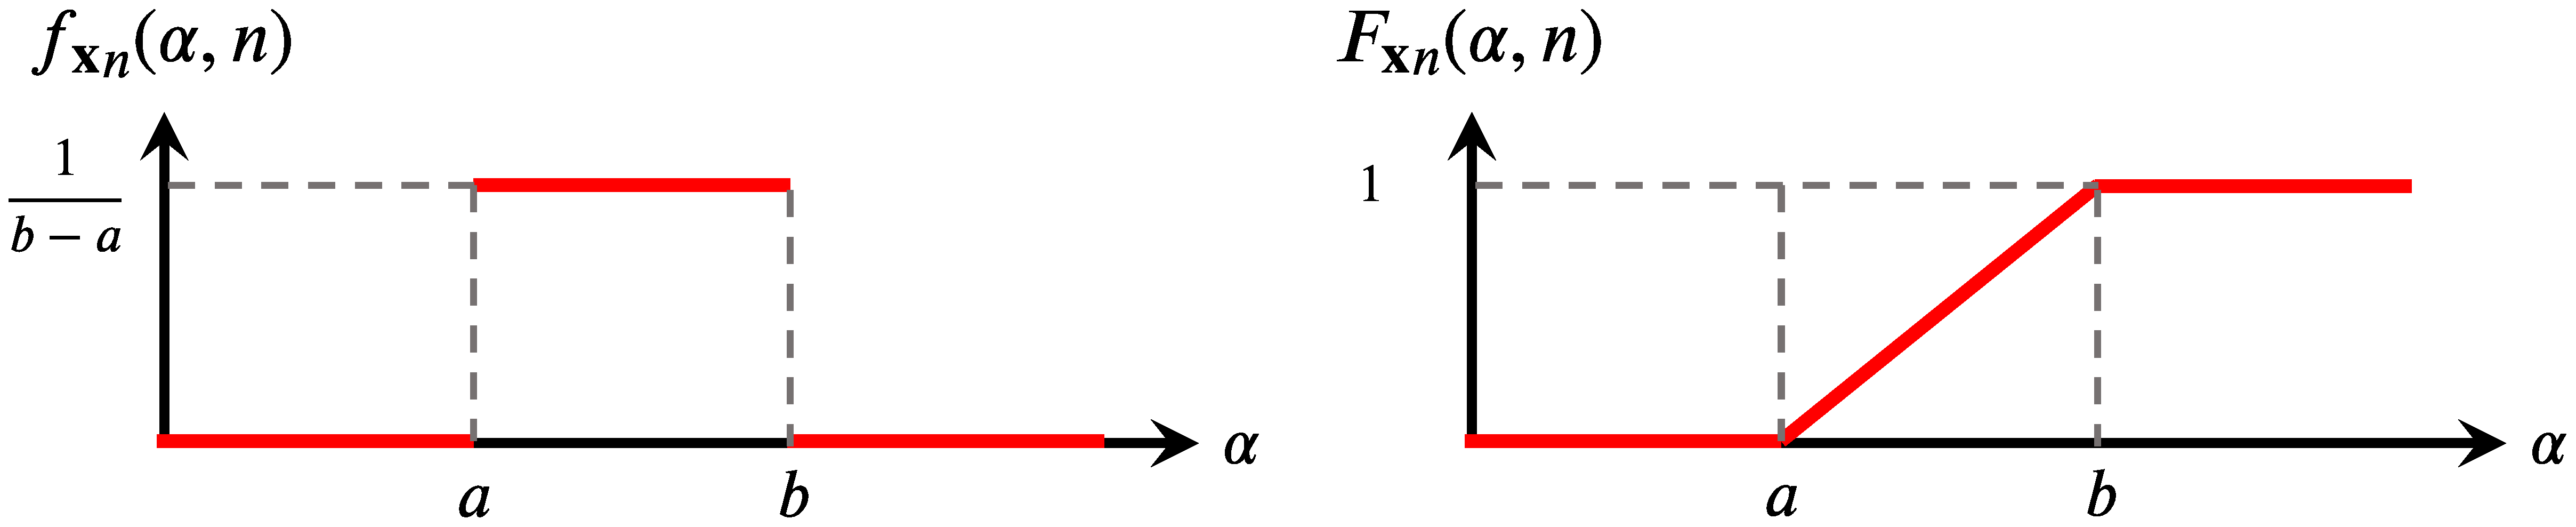
\includegraphics[width=\textwidth]{images/uniform_dist.eps}
                \caption{Plot of the probability density function and probability distribution function of a sample uniform distribution.}
                \label{fig:uniform_dist}
            \end{figure}
        \end{ex}

    \item The \textbf{mean} of a random variable, also the \textbf{expected value}, is defined as
    \[
        m_{\mathbf{x}_n} = \varepsilon\{\mathbf{x}_n\} = \int_{-\infty}^{+\infty} \alpha f_{\mathbf{x}_n}(\alpha, n) \ \mathrm{d}\alpha,
    \]
    where $\varepsilon\{\cdot\}$ denotes the \textbf{expectation operator}. Mathematically,
    \[
        \varepsilon \{ g(\mathbf{x}_n) \} = \int_{-\infty}^{+\infty} g(\alpha) f_{\mathbf{x}_n}(\alpha, n) \ \mathrm{d}\alpha.
    \]

    \begin{ex}{Uniform distribution}
        For the uniform distribution shown in \autoref{ex:uniform_dist}, the mean value is found
        \[
            m_{\mathbf{x}_n} = \int_{a}^{b} \frac{\alpha}{b-a} \ \mathrm{d}\alpha
            = \frac{1}{b-a}\frac{b^2 - a^2}{2} = \frac{a+b}{2}.
        \]
    \end{ex}

    \item The \textbf{variance} is define as
    \[
        \sigma_{\mathbf{x}_n}^2 
        = \varepsilon \{ (\mathbf{x}_n - m_{\mathbf{x}_n})^2 \} 
        = \int_{-\infty}^{+\infty} (\alpha - m_{\mathbf{x}_n})^2 f_{\mathbf{x}_n}(\alpha, n) \ \mathrm{d}\alpha,
    \]
    which is the second-order moment.
    
    \begin{ex}{Uniform distribution}
        For the uniform distribution shown in \autoref{ex:uniform_dist}, the variance is found
        \[
            \sigma_{\mathbf{x}_n}^2
            = \int_{a}^{b} \bigg(\alpha - \underbrace{\frac{a+b}{2}}_{m_{\mathbf{x}_n}}\bigg)^2 \frac{1}{b-a} \ \mathrm{d}\alpha
            = \frac{(b-a)^2}{12}.
        \]
    \end{ex}
\end{enumerate}

%% subsubsection
\subsubsection{Multivariant Probability Functions}
\paragraph{Joint Probability Distribution Function} The \textit{joint} probability distribution function between two random variables $\mathbf{x}_n$,  $\mathbf{x}_m$ is given as 
\[
    F_{\mathbf{x}_n, \mathbf{x}_m}(\alpha_1, \alpha_2, n,m) = P\{\mathbf{x}_n\leq \alpha_1, \mathbf{x}_m \leq \alpha_2\},
\]
The probability distribution function of order $N$ is given as
\[
    F_{\mathbf{x}_{n_1}, ..., \mathbf{x}_{n_N}} (\alpha_1, ..., \alpha_N, n_1, ..., n_N) = P(\mathbf{x}_{n_1} \leq \alpha_{1}, ..., \mathbf{x}_{n_N} \leq \alpha_{N}).
\]

\paragraph{Joint Probability Density Function} The \textit{joint} probability density function between two random variables $\mathbf{x}_n$,  $\mathbf{x}_m$ are given as
\[
    f_{\mathbf{x}_n, \mathbf{x}_m}(\alpha_1, \alpha_2, n,m) = \frac{\partial^2  F_{\mathbf{x}_n, \mathbf{x}_m}(\alpha_1, \alpha_2, n,m)}{\partial \alpha_1 \partial \alpha_2}.
\]
\begin{figure}[H]
    \centering
    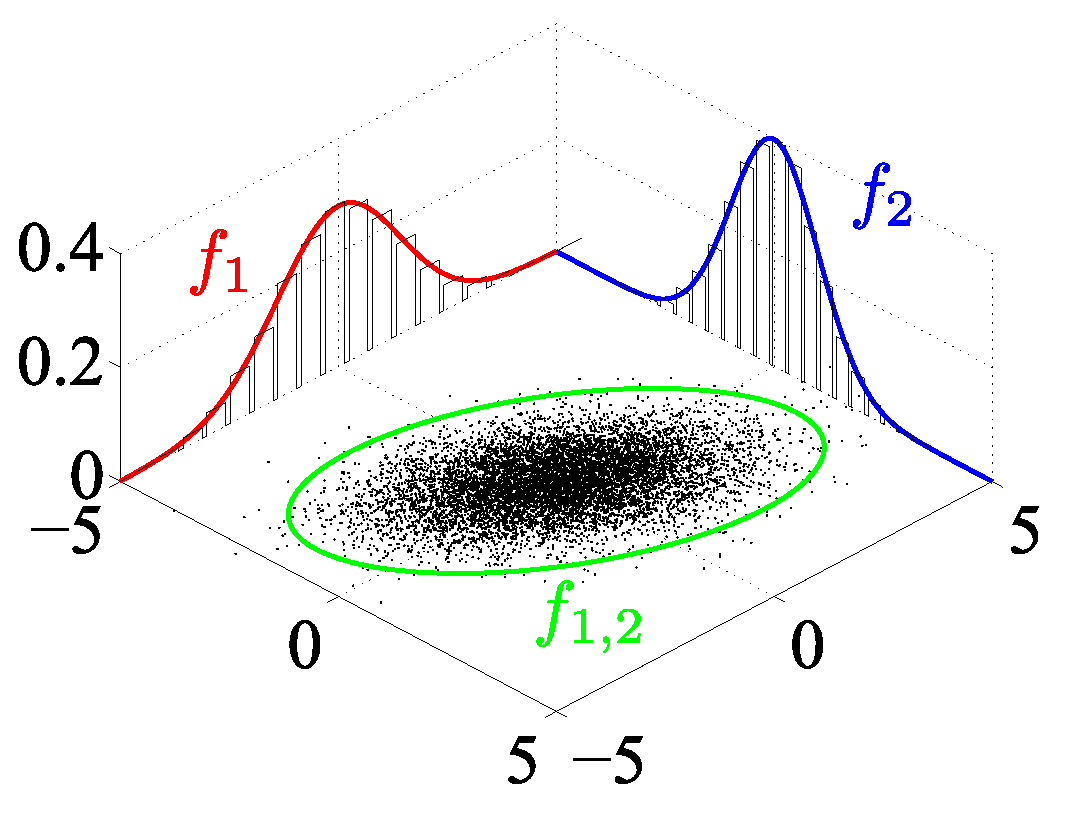
\includegraphics[scale=.5]{images/Multivariate_normal_sample.eps}
    \caption{Many sample observations (black) are shown from a joint probability distribution. Figure adapted and modified based on \href{https://en.wikipedia.org/wiki/Joint_probability_distribution\#/media/File:Multivariate_normal_sample.svg}{WikiPedia}.}
    \label{fig:joint_pdf}
\end{figure}

\paragraph{Statistical Independence} If $\mathbf{x}_n$ and $\mathbf{x}_m$ are \textbf{statistically independent}, or \textbf{uncorrelated}, the joint probability distribution function is equivalent to the product between each single probability distribution function,
\[
    F_{\mathbf{x}_n, \mathbf{x}_m}(\alpha_1, \alpha_2, n,m) = F_{\mathbf{x}_n}(\alpha_1, n)F_{\mathbf{x}_m}(\alpha_2, m),
\]
this also implies that
\[
    f_{\mathbf{x}_n, \mathbf{x}_m}(\alpha_1, \alpha_2, n,m) = f_{\mathbf{x}_n}(\alpha_1, n)f_{\mathbf{x}_m}(\alpha_2, m).
\]
Hence, the mean values are also separable,
\[
    \varepsilon\{\mathbf{x}_n \mathbf{x}_m\} = \varepsilon\{\mathbf{x}_n\}\varepsilon\{\mathbf{x}_m\} = m_{\mathbf{x}_n}m_{\mathbf{x}_m}.
\]

\paragraph{Autocorrelation Function} The autocorrelation function of the random process is defined as the expected value of the product $\mathbf{x}_n \mathbf{x}_m$, denoted by $\phi_{xx}[n,m]$,
\[
    \phi_{xx}[n,m] = \varepsilon\{ \mathbf{x}_n \mathbf{x}_m \}.
\]
\begin{ex}{\textbf{Uniform Distribution}}
    Given a random process with uncorrelated samples of uniform distribution in $[−1,1]$ (\textit{i.e.}, $a=-1$, $b=1$), the autocorrelation function computed with the following steps
    \begin{enumerate}
        \item The mean is found as
        \[
            m_{\mathbf{x}_n} = \frac{a+b}{2} = 0.
        \]

        \item The variance is found as
        \[
            \sigma_{\mathbf{x}_n}^2 = \frac{(b-a)^2}{12} = \frac{1}{3}.
        \]

        \item The autocorrelation between $m$ and $n$ is
        \[
            \phi_{xx}[n,m] 
            = \varepsilon\{ \mathbf{x}_n \mathbf{x}_m \} 
            = 
            \begin{cases}
                \varepsilon\{\mathbf{x}_n\}\varepsilon\{\mathbf{x}_m\}, & \text{if } m \neq n \\
                \varepsilon\{\mathbf{x}_n^2\}, & \text{if } m = n \\
            \end{cases}
            \ = \
            \begin{cases}
                0, & \text{if } m \neq n \\
               \frac{1}{3}, & \text{if } m = n \\
            \end{cases}.
        \]
    \end{enumerate}
\end{ex}

%% subsection
\subsection{Stationarity}
\paragraph{Definition}  A random process is \textbf{stationary} of order $N$, if its joint probability density functions up to order $N$, does not depend on time shifts.\\

For example, $N=2$, the stationarity states that 
\[
    F_{\mathbf{x}_{n+k}}(\alpha, n+k) = F_{\mathbf{x}_{n}}(\alpha, n), \quad \forall k \in \mathbb{Z},
\]
\[
    F_{\mathbf{x}_{n+k}, \mathbf{x}_{m+k}}(\alpha_1, \alpha_2, n+k, m+k) = F_{\mathbf{x}_{n}, \mathbf{x}_{m}}(\alpha_1, \alpha_2, n, m), \quad \forall k \in \mathbb{Z}.
\]

A random process is \textbf{strict-sense stationary} if it is stationary for \textit{any} order $N$.

\subsubsection{Wide-Sense Stationarity}
If the process is stationary of order 2 ($N=2$). The following two properties can be derived,
\begin{enumerate}
    \item its mean does not depend on time, \textit{i.e.},
        \[
            m_{\mathbf{x}_n} = \varepsilon\{\mathbf{x}_n\} = m_{\mathbf{x}}.
        \]
    \item the autocorrelation function depends only on the time difference, 
        \[
            \phi_{xx}[n, m] = \varepsilon\{ \mathbf{x}_n \mathbf{x}_m \} = \int_{-\infty}^{+\infty} \int_{-\infty}^{+\infty} \alpha_1 \alpha_2 f_{\mathbf{x}_n, \mathbf{x}_m} (\alpha_1 \alpha_2, n, m) \ \mathrm{d}\alpha_1 \mathrm{d}\alpha_2,
        \]
        now define $\ell = m-n$ (for which $\ell$ can be regarded as a time shift), we have $m = n + \ell$ 
        \begin{align*}
            \phi_{xx}[n, n+\ell]
            & = \varepsilon\{ \mathbf{x}_n \mathbf{x}_{n+\ell} \} = \int_{-\infty}^{+\infty} \int_{-\infty}^{+\infty} \alpha_1 \alpha_2 f_{\mathbf{x}_n, \mathbf{x}_{n+\ell}} (\alpha_1 \alpha_2, n, {n+\ell}) \ \mathrm{d}\alpha_1 \mathrm{d}\alpha_2\\
            & = \phi_{xx}[\ell].
        \end{align*}
\end{enumerate}
A process with the properties above is referred to as \textbf{wide-sense stationary} (WSS).\\

While the two above properties derive from the definition of stationarity of order 2, \textbf{they do not imply stationarity of order 2}.

\begin{ex}{Uniform Distribution}
A random signal with uncorrelated samples of uniform distribution in $[−a, a]$. The mean of the signal is
\[
    m_{\mathbf{x}_n} = \frac{-a + a}{2} = 0,
\]
and the autocorrelation function is
\[
    \phi_{xx}[n,m] = \frac{a^2}{3} \delta[n-m].
\]
Since the mean does not depend on $n$ and the autocorrelation function depends only on the time lag ($n-m$), the process is WSS.
\end{ex}

\paragraph{Cross-Correlation Function} The cross-correlation function is defined as 
\[
    \phi_{xy} [n,m] = \varepsilon\{\mathbf{x}_n \mathbf{y}_m^*\},
\]
where $\mathbf{x}_n$ and $\mathbf{y}_n$ are two distinct random signals.

%% subsection
\begin{mdframed}[frametitle={Chnage in notation}, nobreak=false]
    From this subsection onward, the random variable at the discrete-time $n$ will be denoted as $x[n]$, instead of $\mathbf{x}_n$.
\end{mdframed}
\subsection{Ergodicity}
\paragraph{Definition}  A process is \textbf{ergodic} for the mean (time-average) if, for any single realization of the process of $x[n]$,
\[
    \langle x[n] \rangle = \lim_{L\to \infty} \frac{1}{2L+1} \sum_{n=-L}^{L} x[n] = \varepsilon\{\mathbf{x}_n\} = m_{x}.
\]

\paragraph{Extended Properties} A process is ergodic for the autocorrelation of
\[
    \langle x[n] x[n+m] \rangle = \lim_{L\to\infty} \frac{1}{2L+1} \sum_{n=-L}^{L} x[n] x[n+m] = \varepsilon\{\mathbf{x}_{n}\mathbf{x}_{n+m}\} = \phi_{xx}[m].
\]

For a WSS random process, ergodic for the autocorrelation function is
\[
    \langle x^2[n] \rangle = \lim_{L\to\infty} \frac{1}{2L+1} \sum_{n=-L}^{L} x^2[n] = \phi_{xx}[0].
\]
The value of the autocorrelation function is zero for an ergodic process corresponds to the power of each of the process realizations.\\

If the process is zero-mean, 
\[
    \lim_{L\to\infty} \frac{1}{2L+1}\sum_{n=-L}^{L} x^2[n] = \phi_{xx}[0] = \sigma_{\mathbf{x}_n}^2.
\]

%% subsubsection
\subsubsection{Variability of Estimates}
In practice, we cannot compute the exact time average since we do not record infinite samples. Thus, we need to make estimates\footnote{such estimated quantities are denoted with a superscript caret, $\widehat{\text{ }}$, to distinguish from the real values} from a finite-length realisation.
\begin{itemize}
    \item Estimating the mean:
    \[
        \widehat{m}_{x} = \frac{1}{L} \sum_{n=0}^{L-1} x[n].
    \]

    \item Estimating the variance:
    \[
        \widehat{\sigma}_x^2 = \frac{1}{L} \sum_{n=0}^{L-1} (x[n] - \widehat{m}_{x})^2.
    \]

    \item Estimating the autocorrelation function:
    \[
        \widehat{\phi}_{xx}[m] = \frac{1}{L}\sum_{n=0}^{L-m-1} \ x[n] \ x[n+m].
    \]
\end{itemize}
The quantities, $\widehat{m}_{x}$, $\widehat{\sigma}_x^2$, and $\widehat{\phi}_{xx}[m]$ are also \textit{random} variables. Hence, we can compute the mean and variability of these estimated quantities. 

\begin{itemize}
    \item The mean of the estimated mean with a finite length:
    \[
        \varepsilon\{\widehat{m}_{x}\} = \varepsilon\bigg\{\frac{1}{L} \sum_{n=0}^{L-1} x[n] \bigg\} = \frac{1}{L} \sum_{n=0}^{L-1} \varepsilon\{x[n]\} = m_x,
    \]
    this means the estimated mean is \textbf{unbiased}.

    \item The variability of the estimated mean with a finite length (for simplicity, assume the true mean $m_x = 0$):
    \[
        \sigma_{\widehat{m}_{x}}^2 = \varepsilon\{(\widehat{m}_{x} - \varepsilon\{\widehat{m}_{x}\})^2\} =  \varepsilon\{(\widehat{m}_{x} - m_x)^2\} = \varepsilon \bigg\{\bigg(\frac{1}{L} \sum_{n=0}^{L-1} x[n]\bigg)^2\bigg\} = \frac{\sigma_x^2}{L}.
    \]
\end{itemize}

\paragraph{Variability in Estimates of the Autocorrelation Function} The estimate of the autocorrelation function in the finite-length realization is a \textbf{biased} estimate.
\[
    \varepsilon\{\widehat{\phi}_{xx}[m]\} = \frac{1}{L}\sum_{n=0}^{L-m-1} \ \varepsilon\{x[n] \ x[n+m] \} = \frac{L-m}{L} \phi_{xx}[m] = \underbrace{(1-\frac{m}{L})}_{\text{deviation from truth}}\phi_{xx}[m].
\]
To fix this, an alternative estimator is proposed to eliminate the bias,
\[
    \widehat{\phi}_{xx}[m] = \frac{1}{L-m}\sum_{n=0}^{L-m-1} \ x[n] \ x[n+m].
\]

%% subsection
\subsection{Power Spectral Density}
\paragraph{Definition} The power spectral density (PSD) of a random process is the ensemble average of the power spectrum of the random process realizations,
\[
    \Phi_{xx} (e^{j\omega}) = \varepsilon \bigg\{ \lim_{L\to\infty} \frac{1}{2L+1} \lvert X_{L}(e^{j\omega}) \rvert^2 \bigg\},
\]
where $X_{L}(e^{j\omega}) = \sum_{n=-L}^{L} x[n] e^{-j\omega n}$ is the Fourier transform of the random variable $x[n]$.

\paragraph{Signal Power} The power spectral density of an ergodic random signal,
\[ 
    \text{signal power} = \frac{1}{2\pi} \int_{-\pi}^{+\pi} \Phi_{xx}(e^{j\omega}) \mathrm{d}\omega
\]
\begin{dv}{}
Start from the RHS of the equation shown above,
\begin{align*}
    & \frac{1}{2\pi} \int_{-\pi}^{+\pi} \Phi_{xx}(e^{j\omega}) \mathrm{d}\omega \\
    & = \frac{1}{2\pi} \int_{-\pi}^{+\pi} \varepsilon \bigg\{ \lim_{L\to \infty} \frac{1} {2L+1} \lvert X_L (e^{j\omega}) \rvert^2 \bigg \} \mathrm{d}\omega \\
    & = \varepsilon \bigg\{ \lim_{L\to \infty} \frac{1} {2L+1} \ \frac{1}{2\pi} \int_{-\pi}^{+\pi} \lvert X_L (e^{j\omega}) \rvert^2 \mathrm{d}\omega \bigg\}.
\end{align*}
By Parseval's theorem:
\[
    \frac{1}{2\pi} \int_{-\infty}^{+\infty} \lvert X(e^{j\omega}) \rvert^2 \mathrm{d}\omega = \sum_{n=-\infty}^{+\infty} \lvert x[n] \rvert^2.
\]
Therefore, 
\[
    \frac{1}{2\pi} \int_{-\pi}^{+\pi} \Phi_{xx}(e^{j\omega}) \mathrm{d}\omega = \varepsilon \bigg\{ \lim_{L\to \infty} \frac{1} {2L+1} \ \sum_{n=-\infty}^{+\infty} \lvert x[n] \rvert^2 \bigg\},
\]
which is the power of the signal.
\end{dv}

\paragraph{Extended Property} The power spectral density of a WSS random process is the discrete-time Fourier transform (DTFT) of the autocorrelation function,
\[
    \Phi_{xx}(e^{j\omega}) = \mathcal{F} \{\phi_{xx}[m]\},
\]
where $\mathcal{F}\{\cdot\}$ denotes the discrete-time Fourier transform.
\begin{dv}{}
\begin{align*}
    \lvert X_{L}(e^{j\omega})\rvert^2 
    & = X_L(e^{j\omega}) X_L^{*}(e^{j\omega}) \\
    & = \sum_{n=-L}^{L} \sum_{r=-L}^{L} x[n] x^{*}[r] e^{-j\omega (n-r)}.
\end{align*}    
Therefore,
\begin{align*}
    \Phi_{xx}(e^{j\omega}) 
    & = \lim_{L\to\infty} \varepsilon \bigg\{ \frac{1}{2L+1} \sum_{n=-L}^{L} \sum_{r=-L}^{L} x[n] x^{*}[r] e^{-j\omega (n-r)} \bigg\} \\
    & = \lim_{L\to \infty} \bigg\{ \frac{1}{2L+1} \sum_{n=-L}^{L} \sum_{r=-L}^{L} \varepsilon \{ x[n] x^{*}[r] e^{-j\omega (n-r)} \} \bigg \}.
\end{align*}
For a WSS random signal,
\[
    \varepsilon \{ x[n] x^{*}[r] \} = \phi_{xx}[n, r] = \phi_{xx}[n-r].
\]
Therefore,
\[
    \Phi_{xx}(e^{j\omega}) = \lim_{L\to \infty} \bigg\{ \frac{1}{2L+1} \sum_{n=-L}^{L} \sum_{r=-L}^{L} \varepsilon \{ \phi_{xx}[n-r] e^{-j\omega (n-r)} \} \bigg \} = \mathcal{F}\{\phi_{xx}[m]\}.
\]
\end{dv}

Therefore, for a WSS and ergodic random signal,
\[
    \Phi(e^{j\omega}) = \mathcal{F} \bigg\{ \lim_{L\to\infty} \frac{1}{2L+1} \sum_{n=-L}^{L} x[n] \ x[n+m] \bigg\}.
\]
This tells us, the PSD is the discrete-time Fourier transform of the autocorrelation function of the process.

%% subsection
\subsection{Periodogram}
\paragraph{Definition} The periodogram is an estimation of the PSD with the limit neglected. 
\[
    \widehat{\Phi}_{xx} (e^{j\omega}) = \frac{1}{2L+1} \lvert X_{L} (e^{j\omega}) \rvert^2
\]
Therefore, it can be shown that the estimation of PSD from the periodogram and from the autocorrelation function is exactly the same:
\[
    \widehat{\Phi}_{xx}(e^{j\omega}) = DTFT \bigg\{ \frac{1}{2L+1} \sum_{n=-L}^{n=L} x[n] \ x[n+m] \bigg\} = DTFT \{ \widehat{\phi}_{xx}[m] \} = \frac{1}{2L+1} \lvert X_{L}(e^{j\omega})\rvert^2
\]
\paragraph{Bias of the Periodogram Estimate}
The expected value of the bias is
\[
    \varepsilon\{\widehat{\Phi}_{xx}(e^{j\omega})\} = \varepsilon \bigg\{ \frac{1}{2L+1} \lvert X_{L}(e^{j\omega})\rvert^2 \bigg\}
\]
This is equivalent to
\[
    x_{L}[n] = 
    \begin{cases}
        x[n], & -L \leq n \leq L \\
        0, & \text{otherwise} \\
    \end{cases}
    = x[n] \cdot w_{2L+1}[n]
    \quad \text{with} \quad 
    w_{2L+1}[n] = 
    \begin{cases}
        1, & -L\leq n\leq L \\
        0, & \text{otherwise} \\
    \end{cases}
\]
Therefore, the periodogram is a biased estimate. The estimate tends to the PSD of the windowed random signal,
\[
    \varepsilon \{ \widehat{\Phi}_{xx}(e^{j\omega}) \} = \Phi_{xx}(e^{j\omega}) * \lvert W_{2L+1}(e^{j\omega}) \rvert^2
\]

\paragraph{Bartlett's Method}
A major problem of the periodogram is \textbf{the variance of the estimate of the PSD is proportional to the square of the PSD value} and \textbf{remains constant with increasing $L$}. \\

To mitigate this issue, we need a compromise between the bias and variance of the estimate. With $N$ recorded samples, one could compromise the bias by dividing $N$ by the number of intervals $K$, yielding $L = N/K$. \\

Thus, we can estimate a periodogram by summing multiple ``piecewise'' periodograms on each interval:

\[
    \widehat{\Phi}_{xx}^B (e^{j\omega}) = \frac{1}{K} \sum_{r=1}^{K} \hat{\Phi}_{x_{r}x_{r}} (e^{j\omega}) \quad \text{with} \quad \hat{\Phi}_{x_{r}x_{r}} = \frac{1}{L} \lvert X_{r} (e^{j\omega}) \rvert^2
\]

The expected values of the periodograms:
\[
    \varepsilon\{\widehat{\Phi}_{xx}^{B} (e^{j\omega}\}
    = \varepsilon\bigg\{ \frac{1}{K} \sum_{r=1}^{K} \widehat{\Phi}_{x_{r}x_{r}} (e^{j\omega}) \bigg\} = \Phi_{xx}(e^{j\omega}) * \lvert W_{2L+1}(e^{j\omega}) \rvert^2
\]
The variance of the periodograms:
\[
    var\{\widehat{\Phi}_{xx}^{B} (e^{j\omega}\} = var \bigg\{ \frac{1}{K} \sum_{r=1}^{K} \widehat{\Phi}_{x_{r}x_{r}} (e^{j\omega}) \bigg\} = \frac{1}{K} var\{\widehat{\Phi}_{xx}(e^{j\omega}) \}
\]
The variance of the estimation decreases as $K$ increases. 

\subsection{Filtering of Random Signals}
\[
    y[n] = x[n] * h[n] = \sum_{k=-\infty}^{+\infty} x[k] h[n-k] = \sum_{k=-\infty}^{+\infty} h[k]x[n-k]
\]
\paragraph{Mean of $y[n]$}
\[
    m_y[n] = \varepsilon\bigg\{ \sum_{k=-\infty}^{+\infty} x[k] h[n-k] \bigg\} = \sum_{k=-\infty}^{+\infty} h[k] \varepsilon\{x[n-k]\} = m_x \sum_{k=-\infty}^{+\infty} h[k]
\]
\paragraph{Autocorrelation function of $y[n]$}
\begin{align*}
    \phi_{yy}[n,\ell] 
    & = \varepsilon \{ y[n] \ y[n+\ell] \} \\
    & = \varepsilon \bigg\{ \sum_{k=-\infty}^{+\infty} h[k]x[n-k] \sum_{k=-\infty}^{+\infty} h[k] x[n+\ell-k] \bigg\} \\
    & = \varepsilon \bigg\{ \sum_{k=-\infty}^{+\infty} \sum_{r=-\infty}^{+\infty} h[k] \ h[r] \ x[n-k] \ x[n+\ell-r] \bigg\} \\
    & = \sum_{k=-\infty}^{+\infty} \sum_{r=-\infty}^{+\infty} h[k] \ h[r] \ \varepsilon \{ x[n-k] \ x[n+\ell-r] \} \\
    & = \sum_{k=-\infty}^{+\infty} \sum_{r=-\infty}^{+\infty} h[k] \ h[r] \ \phi_{xx}[\underbrace{\ell-r+k}_{\text{def.} \ r-k = q}] \\
    & = \sum_{k=-\infty}^{+\infty} \sum_{q=-\infty}^{+\infty} h[k] \ h[k+q] \ \phi_{xx}[\ell-q] \\
    & \hspace{-1cm} (\color{gray}\text{define} \ g[q] = \sum_{k=\infty}^{+\infty}h[k] \ h[k+q] = h[q] * h[-q]) \\
    & = \sum_{q=-\infty}^{+\infty} g[q] \phi_{xx}[\ell-q] = g[\ell]*\phi_{xx}[\ell] = \phi_{yy}[\ell]
\end{align*}

\paragraph{PSD of $y[n]$}
The PSD of $y[n]$ is the discrete-time FT of the autocorrelation function $\phi_{yy}[\ell]$,
\[
    \phi_{yy}[\ell] = g[\ell] * \phi_{xx}[\ell]
\]
with $g[q] = h[q] * h[-q]$,
\[  
    \Phi_{yy}(e^{j\omega}) = DTFT\{ g[\ell] * \phi_{xx}[\ell] \} = G(e^{j\omega} \cdot \Phi_{xx} (e^{j\omega})
\]
with 
\[
    G(e^{j\omega}) = DTFT \{ h[q] *h[-q] \} = H(e^{j\omega}) \cdot H^{*}(e^{j\omega}) = \lvert H(e^{j\omega}) \rvert^2
\]
Therefore, 
\[
    \Phi_{yy}(e^{j\omega}) = \lvert H(e^{j\omega}) \rvert^2 \cdot \Phi_{xx}(e^{j\omega})
\]

\subsection{Linear Predictor}
The mean square error for the linear predictor
\[
    \varepsilon\{\lvert e[n] \rvert^2\} = \varepsilon \bigg\{ \bigg( x[n] - \sum_{k=1}^{N} a_k x[n-k] \bigg)^2 \bigg\} = \phi_{xx}[0] + \sum_{k=1}^{N}\sum_{r=1}^N a_k a_r \phi_{xx}[r-k] - 2 \sum_{k=1}^N a_k \phi_{xx}[k]
\]
Minimising the MSE,
\[
    \frac{\partial \varepsilon\{\lvert e[n] \rvert^2\}}{\partial a_{\ell}} = 0, \quad \ell = 1, 2,..., N
\]
with
\[
    \frac{\partial \varepsilon\{\lvert e[n] \rvert^2\}}{\partial a_{\ell}} = 2\sum_{k=1}^N a_k \phi_{xx}[k-\ell] - 2\phi_{xx}[\ell]
\]
Hence
\[
    2\sum_{k=1}^N a_k \phi_{xx}[k-\ell] - 2\phi_{xx}[\ell] = 0 
    \quad \Rightarrow \quad
    \boxed{\sum_{k=1}^N a_k \phi_{xx}[k-\ell] = \phi_{xx}[\ell]}
\]
which is equivalent to
\[
    \varepsilon \{e[n] \ x[n-k] \} = 0, \quad k = 1, 2, ..., N
\]
The error in the linear prediction can thus be seen as part of the innovation of the process that is not contained in the previous $N$ samples.

\subsection{Modelling}
Consider an LTI system with the input $u[n]$, system function $H(e^{j\omega})$, and output $x[n]$, for which $u[n]$ is a white random process.
\begin{figure}[H]
    \centering
    \begin{tikzpicture}[auto, node distance=2.2cm, >=Latex]
        % Nodes
        \node (input) {$u[n]$};
        \node [draw, line width=0.25mm, rectangle, minimum width=1.5cm, minimum height=0.7cm, right=.7cm of input] (block1) {$H(e^{^{j\omega}})$};
        \node [right=0.7cm of block1] (output) {$x[n]$};
        % Arrows
        \draw[line width=0.25mm, ->] (input) -- (block1);
        \draw[line width=0.25mm, ->] (block1) -- (output);
    \end{tikzpicture}
\end{figure}
Recall that in Section 5, the system response can be expressed using the difference equation
\[
    x[n] = \sum_{k=1}^{N} a_{k}x[n-k] + \sum_{k=0}^{M} b_{k}u[n-k].
\]
Further, the system function corresponding to the difference form is
\[
    H(z) = \frac{\sum_{k=0}^{M} b_{k} z^{-k}}{1-\sum_{k=1}^{N} a_{k} z^{-k}}
    \quad \Leftrightarrow \quad
    H(e^{j\omega}) = \frac{\sum_{k=0}^M b_k e^{-j\omega k}}{1-\sum_{k=1}^N a_k e^{-j\omega k}},
\]

Therefore, the power spectrum of $x[n]$ is found
\[
    \Phi_{xx}(e^{j\omega}) = \sigma_u^2 \cdot \lvert H(e^{j\omega}) \rvert^2 = \sigma_u^2 \cdot \bigg \lvert \frac{\sum_{k=0}^M b_k e^{-j\omega k}}{1-\sum_{k=1}^N a_k e^{-j\omega k}} \bigg\rvert^2 . 
\]
This model is known as the \textbf{autoregressive, moving average} model (ARMA).
\begin{itemize}
    \item By setting $M = 0$: autoregressive (AR) model
    \[
        x[n] = \sum_{k=1}^{N} a_{k}x[n-k] + u[n]
        \quad \text{and} \quad
        \Phi_{xx}(e^{j\omega}) = \sigma_u^2 \cdot  \frac{1}{\lvert 1-\sum_{k=1}^N a_k e^{-j\omega k}\rvert^2}
    \]

    \item By setting $N = 0$: moving average (MA) model
    \[
        x[n] = \sum_{k=0}^{M} b_{k}u[n-k]
        \quad \text{and} \quad
        \Phi_{xx}(e^{j\omega}) = \sigma_u^2 \cdot  \left\vert \sum_{k=0}^M b_k e^{-j\omega k} \right\vert^2
    \]
\end{itemize}

\subsection{Example Questions}
%==============================================%
\begin{q}{}
Let $x[n]$ and $y[n]$ be stationary, uncorrelated to each other, discrete-time random processes with mean values $m_x$ and $m_y$, respectively, and $w[n] = x[n] \cdot y[n]$. The mean value of $w[n]$ is

\begin{enumerate}[label=(\alph*)]
    \item Always zero
    \item Zero only of $m_x = 0$ and $m_y = 0$
    \item Zero if $m_x = 0$ or $m_y = 0$
    \item Always smaller than $m_x$
    \item Always smaller than $m_y$
\end{enumerate}
\begin{flushright}
    \begin{blueenv}
        ANS: (c)
    \end{blueenv}
\end{flushright}
\end{q}
%==============================================%
\begin{q}{}
Let $x[n]$ and $y[n]$ be two stationary, zero-mean, uncorrelated to each other, discrete-time random processes, with variances $\sigma_x^2$ and $\sigma_y^2$, and power spectra $\Phi_{xx}(e^{j\omega})$ and $\Phi_{yy}(e^{j\omega})$, respectively.\\

Let's define the random process $w[n] = x[n] + 2y[n]$, with variance $\sigma_w^2$ and power spectrum $\Phi_{ww}(e^{j\omega})$. Which of the following relations is always correct?

\begin{enumerate}[label=(\alph*)]
    \item $\Phi_{ww}(e^{j\omega}) = 2\Phi_{xx}(e^{j\omega}) \Phi_{yy}(e^{j\omega})$
    \item $\Phi_{ww}(e^{j\omega}) = \Phi_{xx}(e^{j\omega}) + 2\Phi_{yy}(e^{j\omega})$
    \item $\sigma_w^2 = \sigma_x^2 + 2\sigma_y^2$
    \item $\sigma_w^2 = \sigma_x^2 + 4\sigma_y^2$
    \item $\sigma_w^2 = 0$
\end{enumerate}
\begin{flushright}
    \begin{blueenv}
        ANS: (d)
    \end{blueenv}
\end{flushright}
\end{q}
%==============================================%
\begin{q}{}
Consider the wide-sense stationary (WSS) random process $x[n]$, with autocorrelation function $\phi_{xx}[\ell]$ and unitary variance. The autocorrelation function $\phi_{xx}[\ell]$ is equal to zero for all values of the time lag $\ell$ for which $|\ell| \geq 3$. The random process $x[n]$ is down-sampled by a factor of 3 to obtain the down-sampled random process $e[n]$. Which of the following expressions/statements for the autocorrelation function $\phi_{ee}[\ell]$ of $e[n]$ is correct?

\begin{enumerate}[label=(\alph*)]
    \item $\phi_{ee}[\ell] = \delta[\ell]$
    \item $\phi_{ee}[\ell] = \phi_{xx}[\ell]$
    \item $\phi_{ee}[\ell] = 3\phi_{xx}[\ell]$
    \item $\phi_{ee}[\ell] = 0$ for all values of $\ell$
    \item $\phi_{ee}[\ell]$ is an odd function
\end{enumerate}

\begin{flushright}
    \begin{blueenv}
        ANS: (d)
    \end{blueenv}
\end{flushright}
\end{q}
%==============================================%
\begin{q}{}
Consider the cascade of two LTI systems as represented below:
\begin{figure}[H]
    \centering
    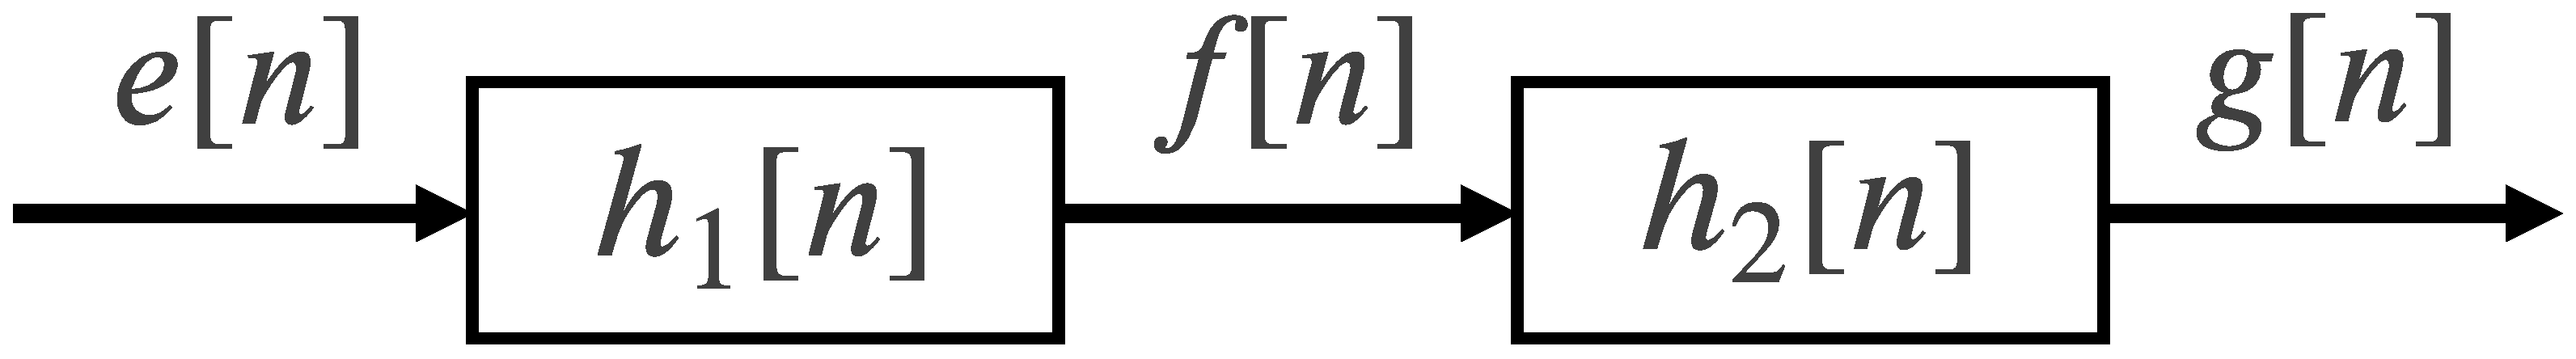
\includegraphics[width=.5\textwidth]{images/random_proc_ex.eps}
\end{figure}
where $h_1[n] = \delta[n] - \delta[n-1]$ and $\displaystyle H_2(e^{j\omega}) = \begin{cases}
1, \quad \lvert \omega \rvert < \omega_c \\
0, \quad \omega_c < \lvert \omega \rvert \leq \pi
\end{cases}
$ with $\omega_{c} < \pi$. Moreover, $e[n]$ is a stationary, white random signal, with zero mean and power $\sigma_{e}^2 = 1$.

\begin{enumerate}[label=(\alph*)]
    \item Find and plot the power spectrum $\Phi_{ff}(e^{j\omega})$ of the random signal $f[n]$.

    \begin{flushright}
        \begin{blueenv}
            ANS: $\Phi_{ff}(e^{j\omega}) = 2 (1 - \cos\omega)$.
        \end{blueenv}
    \end{flushright}

    \item Find the autocorrelation function $\phi_{ff}[\ell]$ of the random signal.
    \begin{flushright}
        \begin{blueenv}
            ANS: $\phi_{ff}[\ell] = 2\delta[\ell] - \delta[\ell-1] - \delta[\ell + 1]$.
        \end{blueenv}
    \end{flushright}

    \item Find the power spectrum $\Phi_{gg}(e^{j\omega})$ of the random signal $g[n]$ as a function of $\omega_c$ (cut-off frequency of the second LTI system).
    \begin{flushright}
        \begin{blueenv}
            ANS: $\phi_{gg}[\ell] = 
            \begin{cases}
            2(1-\cos\omega), & \lvert \omega \rvert \leq \omega_c \\
            0, & \omega_c < \lvert \omega \rvert \leq \pi
            \end{cases}$.
        \end{blueenv}
    \end{flushright}

    \item Find the power $\sigma_{e}^{2}$ of the random signal $g[n]$ as a function of $\omega_c$ (cut-off frequency of the second LTI system).
    \begin{flushright}
        \begin{blueenv}
            ANS: $\sigma_{g}^2 = \dfrac{2\omega_c}{\pi}$.
        \end{blueenv}
    \end{flushright}
\end{enumerate}

% \begin{blueenv}
% \paragraph{Answer (a)}
% \[
%     \Phi_{ff}(e^{j\omega}) = \Phi_{ee}(e^{j\omega}) \cdot \lvert H_1(e^{j\omega})\rvert^2,
% \]
% with
% \begin{itemize}
%     \item $\Phi_{ee}(e^{j\omega}) = 1$, 
%     \item $h_1[n] \ \xrightarrow[]{\mathcal{F}}H_1(e^{j\omega}) = 1 - e^{-j\omega} \quad \Rightarrow \quad \lvert H_1(e^{j\omega})\rvert^2 = 2 (1 - \cos\omega)$.
% \end{itemize}
% Hence, $\Phi_{ff}(e^{j\omega}) = 2 (1 - \cos\omega)$.

% \paragraph{Answer (b)} Given
% \[
%     f[n] = e[n] - e[n-1],
% \]
% hence,
% \begin{align*}
%     \phi_{ff}[\ell] 
%     & = \varepsilon \{f[n] \ f[n+\ell]\} \\
%     & = \varepsilon \{(e[n] - e[n-1])(e[n+\ell] - e[n+\ell-1])\} \\
%     & = 2 \phi_{ee}[\ell] - \phi_{ee}[\ell-1] - \phi_{ee}[\ell+1] \\
%     & = 2\delta[\ell] - \delta[\ell-1] - \delta[\ell + 1]
% \end{align*}

% \paragraph{Answer (c)}
% \[
%     \Phi_{gg}(e^{j\omega}) = \Phi_{ff}(e^{j\omega}) \lvert H_2(e^{j\omega}) \rvert^2 = 
%     \begin{cases}
%         2(1-\cos\omega), & \lvert \omega \rvert \leq \omega_c \\
%         0, & \omega_c < \lvert \omega \rvert \leq \pi
%     \end{cases}
% \]

% \paragraph{Answer (d)}
% \begin{align*}
%     \sigma_{g}^2
%     & = \frac{1}{2\pi} \int_{-\infty}^{+\infty} \Phi_{gg}(e^{j\omega}) \mathrm{d}\omega \\
%     & = \frac{1}{2\pi} \int_{-\omega_c}^{+\omega_c} 2(1-\cos\omega) \mathrm{d}\omega \\
%     & = \frac{1}{2\pi} (4\omega_c - 2\sin\omega_c + 2\sin\omega_c) \\
%     & = \frac{2\omega_c}{\pi}
% \end{align*}
% \end{blueenv}
    
\end{q}